\documentclass[twoside]{book}

% Packages required by doxygen
\usepackage{fixltx2e}
\usepackage{calc}
\usepackage{doxygen}
\usepackage[export]{adjustbox} % also loads graphicx
\usepackage{graphicx}
\usepackage[utf8]{inputenc}
\usepackage{makeidx}
\usepackage{multicol}
\usepackage{multirow}
\PassOptionsToPackage{warn}{textcomp}
\usepackage{textcomp}
\usepackage[nointegrals]{wasysym}
\usepackage[table]{xcolor}

% Font selection
\usepackage[T1]{fontenc}
\usepackage[scaled=.90]{helvet}
\usepackage{courier}
\usepackage{amssymb}
\usepackage{sectsty}
\renewcommand{\familydefault}{\sfdefault}
\allsectionsfont{%
  \fontseries{bc}\selectfont%
  \color{darkgray}%
}
\renewcommand{\DoxyLabelFont}{%
  \fontseries{bc}\selectfont%
  \color{darkgray}%
}
\newcommand{\+}{\discretionary{\mbox{\scriptsize$\hookleftarrow$}}{}{}}

% Page & text layout
\usepackage{geometry}
\geometry{%
  a4paper,%
  top=2.5cm,%
  bottom=2.5cm,%
  left=2.5cm,%
  right=2.5cm%
}
\tolerance=750
\hfuzz=15pt
\hbadness=750
\setlength{\emergencystretch}{15pt}
\setlength{\parindent}{0cm}
\setlength{\parskip}{3ex plus 2ex minus 2ex}
\makeatletter
\renewcommand{\paragraph}{%
  \@startsection{paragraph}{4}{0ex}{-1.0ex}{1.0ex}{%
    \normalfont\normalsize\bfseries\SS@parafont%
  }%
}
\renewcommand{\subparagraph}{%
  \@startsection{subparagraph}{5}{0ex}{-1.0ex}{1.0ex}{%
    \normalfont\normalsize\bfseries\SS@subparafont%
  }%
}
\makeatother

% Headers & footers
\usepackage{fancyhdr}
\pagestyle{fancyplain}
\fancyhead[LE]{\fancyplain{}{\bfseries\thepage}}
\fancyhead[CE]{\fancyplain{}{}}
\fancyhead[RE]{\fancyplain{}{\bfseries\leftmark}}
\fancyhead[LO]{\fancyplain{}{\bfseries\rightmark}}
\fancyhead[CO]{\fancyplain{}{}}
\fancyhead[RO]{\fancyplain{}{\bfseries\thepage}}
\fancyfoot[LE]{\fancyplain{}{}}
\fancyfoot[CE]{\fancyplain{}{}}
\fancyfoot[RE]{\fancyplain{}{\bfseries\scriptsize Generated by Doxygen }}
\fancyfoot[LO]{\fancyplain{}{\bfseries\scriptsize Generated by Doxygen }}
\fancyfoot[CO]{\fancyplain{}{}}
\fancyfoot[RO]{\fancyplain{}{}}
\renewcommand{\footrulewidth}{0.4pt}
\renewcommand{\chaptermark}[1]{%
  \markboth{#1}{}%
}
\renewcommand{\sectionmark}[1]{%
  \markright{\thesection\ #1}%
}

% Indices & bibliography
\usepackage{natbib}
\usepackage[titles]{tocloft}
\setcounter{tocdepth}{3}
\setcounter{secnumdepth}{5}
\makeindex

% Hyperlinks (required, but should be loaded last)
\usepackage{ifpdf}
\ifpdf
  \usepackage[pdftex,pagebackref=true]{hyperref}
\else
  \usepackage[ps2pdf,pagebackref=true]{hyperref}
\fi
\hypersetup{%
  colorlinks=true,%
  linkcolor=blue,%
  citecolor=blue,%
  unicode%
}

% Custom commands
\newcommand{\clearemptydoublepage}{%
  \newpage{\pagestyle{empty}\cleardoublepage}%
}

\usepackage{caption}
\captionsetup{labelsep=space,justification=centering,font={bf},singlelinecheck=off,skip=4pt,position=top}

%===== C O N T E N T S =====

\begin{document}

% Titlepage & ToC
\hypersetup{pageanchor=false,
             bookmarksnumbered=true,
             pdfencoding=unicode
            }
\pagenumbering{alph}
\begin{titlepage}
\vspace*{7cm}
\begin{center}%
{\Large My Project }\\
\vspace*{1cm}
{\large Generated by Doxygen 1.8.13}\\
\end{center}
\end{titlepage}
\clearemptydoublepage
\pagenumbering{roman}
\tableofcontents
\clearemptydoublepage
\pagenumbering{arabic}
\hypersetup{pageanchor=true}

%--- Begin generated contents ---
\chapter{L\+I2-\/\+P\+L8-\/\+Grp12}
\label{md_README}
\Hypertarget{md_README}
Projeto no âmbito da disciplina de Laboratórios de Informática 2. O objetivo é desenvolver o jogo \char`\"{}\+Rastros\char`\"{} na linguagem C. Projeto realizado por\+: Laura Nunes Rodrigues a93169; Luís Miguel Teixeira Fernandes a88539; Mariana Filipa da Silva Rodrigues a93306. Alunos do P\+L8, grupo 12. 
\chapter{Class Index}
\section{Class List}
Here are the classes, structs, unions and interfaces with brief descriptions\+:\begin{DoxyCompactList}
\item\contentsline{section}{\hyperlink{structCOORDENADA}{C\+O\+O\+R\+D\+E\+N\+A\+DA} \\*Tipo de dados para as coordenadas }{\pageref{structCOORDENADA}}{}
\item\contentsline{section}{\hyperlink{structESTADO}{E\+S\+T\+A\+DO} \\*Tipo de dados para o estado }{\pageref{structESTADO}}{}
\item\contentsline{section}{\hyperlink{structJOGADA}{J\+O\+G\+A\+DA} \\*Tipo de dados para a jogada }{\pageref{structJOGADA}}{}
\end{DoxyCompactList}

\chapter{Class Documentation}
\hypertarget{structCOORDENADA}{}\section{C\+O\+O\+R\+D\+E\+N\+A\+DA Struct Reference}
\label{structCOORDENADA}\index{C\+O\+O\+R\+D\+E\+N\+A\+DA@{C\+O\+O\+R\+D\+E\+N\+A\+DA}}
\subsection*{Public Attributes}
\begin{DoxyCompactItemize}
\item 
\mbox{\Hypertarget{structCOORDENADA_adfbc8d4856ce807139fdf62e00aed29a}\label{structCOORDENADA_adfbc8d4856ce807139fdf62e00aed29a}} 
int {\bfseries coluna}
\item 
\mbox{\Hypertarget{structCOORDENADA_aefe14bcc5a066ac3b21500cc3d28c06f}\label{structCOORDENADA_aefe14bcc5a066ac3b21500cc3d28c06f}} 
int {\bfseries linha}
\end{DoxyCompactItemize}


The documentation for this struct was generated from the following file\+:\begin{DoxyCompactItemize}
\item 
Camada\+\_\+dados.\+h\end{DoxyCompactItemize}

\hypertarget{structESTADO}{}\section{E\+S\+T\+A\+DO Struct Reference}
\label{structESTADO}\index{E\+S\+T\+A\+DO@{E\+S\+T\+A\+DO}}


Tipo de dados para o estado.  




{\ttfamily \#include $<$Camada\+\_\+dados.\+h$>$}



Collaboration diagram for E\+S\+T\+A\+DO\+:
\nopagebreak
\begin{figure}[H]
\begin{center}
\leavevmode
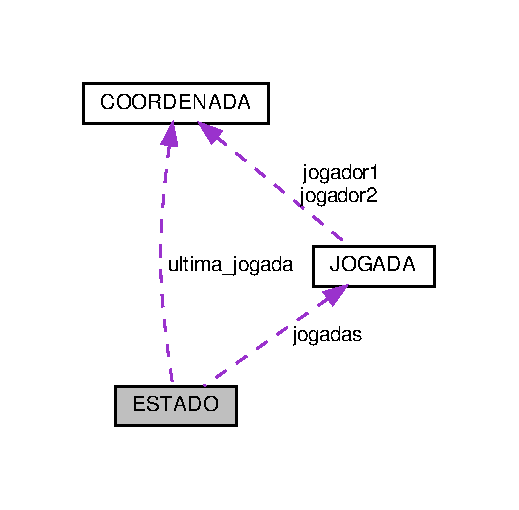
\includegraphics[width=249pt]{structESTADO__coll__graph}
\end{center}
\end{figure}
\subsection*{Public Attributes}
\begin{DoxyCompactItemize}
\item 
\hyperlink{Camada__dados_8h_aba91601f16d4c485b2d9b8c429f27039}{C\+A\+SA} \hyperlink{structESTADO_ab56f0f1be16954d3768b4174d14c087d}{tab} \mbox{[}8\mbox{]}\mbox{[}8\mbox{]}
\item 
\hyperlink{structCOORDENADA}{C\+O\+O\+R\+D\+E\+N\+A\+DA} \hyperlink{structESTADO_a4896a5c5c1f40b43fb795623327e3f47}{ultima\+\_\+jogada}
\item 
\hyperlink{Camada__dados_8h_a94c221d29a1760f008b7834093259b7d}{J\+O\+G\+A\+D\+AS} \hyperlink{structESTADO_afae43b87a488fad0f2b56a18bad31d18}{jogadas}
\item 
int \hyperlink{structESTADO_a261495728744647e618b4e623f5a4b7a}{num\+\_\+jogadas}
\item 
int \hyperlink{structESTADO_a5dd28e2e68b7aef2b6b7ea88e02eff58}{jogador\+\_\+atual}
\item 
int \hyperlink{structESTADO_a8d478f3546194c1666c6e390c8aaf1cb}{num\+\_\+movimentos}
\item 
int \hyperlink{structESTADO_aceee2863ecd183efc410fb079a576cba}{alt\+\_\+pos}
\end{DoxyCompactItemize}


\subsection{Detailed Description}
Tipo de dados para o estado. 

\subsection{Member Data Documentation}
\mbox{\Hypertarget{structESTADO_aceee2863ecd183efc410fb079a576cba}\label{structESTADO_aceee2863ecd183efc410fb079a576cba}} 
\index{E\+S\+T\+A\+DO@{E\+S\+T\+A\+DO}!alt\+\_\+pos@{alt\+\_\+pos}}
\index{alt\+\_\+pos@{alt\+\_\+pos}!E\+S\+T\+A\+DO@{E\+S\+T\+A\+DO}}
\subsubsection{\texorpdfstring{alt\+\_\+pos}{alt\_pos}}
{\footnotesize\ttfamily int E\+S\+T\+A\+D\+O\+::alt\+\_\+pos}

Jogada anterior foi pos \mbox{\Hypertarget{structESTADO_afae43b87a488fad0f2b56a18bad31d18}\label{structESTADO_afae43b87a488fad0f2b56a18bad31d18}} 
\index{E\+S\+T\+A\+DO@{E\+S\+T\+A\+DO}!jogadas@{jogadas}}
\index{jogadas@{jogadas}!E\+S\+T\+A\+DO@{E\+S\+T\+A\+DO}}
\subsubsection{\texorpdfstring{jogadas}{jogadas}}
{\footnotesize\ttfamily \hyperlink{Camada__dados_8h_a94c221d29a1760f008b7834093259b7d}{J\+O\+G\+A\+D\+AS} E\+S\+T\+A\+D\+O\+::jogadas}

As jogadas \mbox{\Hypertarget{structESTADO_a5dd28e2e68b7aef2b6b7ea88e02eff58}\label{structESTADO_a5dd28e2e68b7aef2b6b7ea88e02eff58}} 
\index{E\+S\+T\+A\+DO@{E\+S\+T\+A\+DO}!jogador\+\_\+atual@{jogador\+\_\+atual}}
\index{jogador\+\_\+atual@{jogador\+\_\+atual}!E\+S\+T\+A\+DO@{E\+S\+T\+A\+DO}}
\subsubsection{\texorpdfstring{jogador\+\_\+atual}{jogador\_atual}}
{\footnotesize\ttfamily int E\+S\+T\+A\+D\+O\+::jogador\+\_\+atual}

O jogador atual \mbox{\Hypertarget{structESTADO_a261495728744647e618b4e623f5a4b7a}\label{structESTADO_a261495728744647e618b4e623f5a4b7a}} 
\index{E\+S\+T\+A\+DO@{E\+S\+T\+A\+DO}!num\+\_\+jogadas@{num\+\_\+jogadas}}
\index{num\+\_\+jogadas@{num\+\_\+jogadas}!E\+S\+T\+A\+DO@{E\+S\+T\+A\+DO}}
\subsubsection{\texorpdfstring{num\+\_\+jogadas}{num\_jogadas}}
{\footnotesize\ttfamily int E\+S\+T\+A\+D\+O\+::num\+\_\+jogadas}

O número das jogadas, usado no prompt \mbox{\Hypertarget{structESTADO_a8d478f3546194c1666c6e390c8aaf1cb}\label{structESTADO_a8d478f3546194c1666c6e390c8aaf1cb}} 
\index{E\+S\+T\+A\+DO@{E\+S\+T\+A\+DO}!num\+\_\+movimentos@{num\+\_\+movimentos}}
\index{num\+\_\+movimentos@{num\+\_\+movimentos}!E\+S\+T\+A\+DO@{E\+S\+T\+A\+DO}}
\subsubsection{\texorpdfstring{num\+\_\+movimentos}{num\_movimentos}}
{\footnotesize\ttfamily int E\+S\+T\+A\+D\+O\+::num\+\_\+movimentos}

Número de movimentos \mbox{\Hypertarget{structESTADO_ab56f0f1be16954d3768b4174d14c087d}\label{structESTADO_ab56f0f1be16954d3768b4174d14c087d}} 
\index{E\+S\+T\+A\+DO@{E\+S\+T\+A\+DO}!tab@{tab}}
\index{tab@{tab}!E\+S\+T\+A\+DO@{E\+S\+T\+A\+DO}}
\subsubsection{\texorpdfstring{tab}{tab}}
{\footnotesize\ttfamily \hyperlink{Camada__dados_8h_aba91601f16d4c485b2d9b8c429f27039}{C\+A\+SA} E\+S\+T\+A\+D\+O\+::tab\mbox{[}8\mbox{]}\mbox{[}8\mbox{]}}

O tabuleiro \mbox{\Hypertarget{structESTADO_a4896a5c5c1f40b43fb795623327e3f47}\label{structESTADO_a4896a5c5c1f40b43fb795623327e3f47}} 
\index{E\+S\+T\+A\+DO@{E\+S\+T\+A\+DO}!ultima\+\_\+jogada@{ultima\+\_\+jogada}}
\index{ultima\+\_\+jogada@{ultima\+\_\+jogada}!E\+S\+T\+A\+DO@{E\+S\+T\+A\+DO}}
\subsubsection{\texorpdfstring{ultima\+\_\+jogada}{ultima\_jogada}}
{\footnotesize\ttfamily \hyperlink{structCOORDENADA}{C\+O\+O\+R\+D\+E\+N\+A\+DA} E\+S\+T\+A\+D\+O\+::ultima\+\_\+jogada}

A coordenada da última jogada 

The documentation for this struct was generated from the following file\+:\begin{DoxyCompactItemize}
\item 
\hyperlink{Camada__dados_8h}{Camada\+\_\+dados.\+h}\end{DoxyCompactItemize}

\hypertarget{structJOGADA}{}\section{J\+O\+G\+A\+DA Struct Reference}
\label{structJOGADA}\index{J\+O\+G\+A\+DA@{J\+O\+G\+A\+DA}}


Tipo de dados para a jogada.  




{\ttfamily \#include $<$Camada\+\_\+dados.\+h$>$}



Collaboration diagram for J\+O\+G\+A\+DA\+:
\nopagebreak
\begin{figure}[H]
\begin{center}
\leavevmode
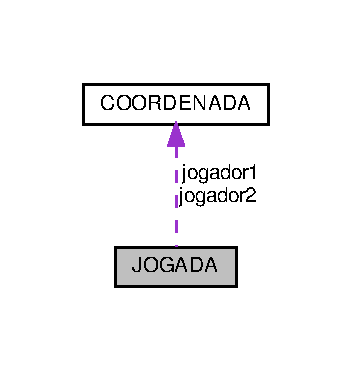
\includegraphics[width=169pt]{structJOGADA__coll__graph}
\end{center}
\end{figure}
\subsection*{Public Attributes}
\begin{DoxyCompactItemize}
\item 
\mbox{\Hypertarget{structJOGADA_a93d9306cb0c49b66b7d9a615bffe0149}\label{structJOGADA_a93d9306cb0c49b66b7d9a615bffe0149}} 
\hyperlink{structCOORDENADA}{C\+O\+O\+R\+D\+E\+N\+A\+DA} {\bfseries jogador1}
\item 
\mbox{\Hypertarget{structJOGADA_ab46b16dfbdc7f2af9430c8dcdac0914b}\label{structJOGADA_ab46b16dfbdc7f2af9430c8dcdac0914b}} 
\hyperlink{structCOORDENADA}{C\+O\+O\+R\+D\+E\+N\+A\+DA} {\bfseries jogador2}
\end{DoxyCompactItemize}


\subsection{Detailed Description}
Tipo de dados para a jogada. 

The documentation for this struct was generated from the following file\+:\begin{DoxyCompactItemize}
\item 
\hyperlink{Camada__dados_8h}{Camada\+\_\+dados.\+h}\end{DoxyCompactItemize}

%--- End generated contents ---

% Index
\backmatter
\newpage
\phantomsection
\clearemptydoublepage
\addcontentsline{toc}{chapter}{Index}
\printindex

\end{document}
